\chapter[Analiza zmogljivosti obla"cne storitve DigitalOcean]{Analiza zmogljivosti obla"cne storitve DigitalOcean}

\pagestyle{fancy}
\fancyhf{}
\fancyhead[LE,RO]{\thepage}
\fancyhead[RE,LO]{\leftmark}

\huge "Ziga Kokelj, Tadej Hiti,\\Miha Bizjak, Matej Kristan
\normalsize
\bigskip

\section{Opis problema} \label{8_opis_problema}
\noindent V zadnjem desetletju se na vseh podro"cjih ra"cunalni"stva vse bolj uveljavljajo obla"cne storitve in koncept odjemalec - stre"znik (angl. client - server). Z ve"canjem hitrosti internetnih povezav kon"cne delovne to"cke(predvsem osebni ra"cunalniki) izgubljajo del svojih primarnih funkcij. Hranjenje in obdelavo podatkov vse bolj prepu"scajo obla"cnim storitvam. V na"si analizi smo se osredoto"cili na obdelavo podatkov na strani stre"znika. Za breme smo izbrali datoteke razli"cnih velikosti, ki vsebujejo naklju"cna "stevila. Te datoteke odlemalci po"slejo na stre"znik, ki jih mora urediti v nara"scajocem vrstnem redu in poslati nazaj.  Na sliki \ref{8_opis_problema} je grafi"cen prikaz opisanega problema. Na"se testiranje bo obsegalo merjenje  "case "cakanja  klientov na urejeno datoteko ter merjenje obremenjenosti stre"znika. 

\begin{figure}
  \centering
    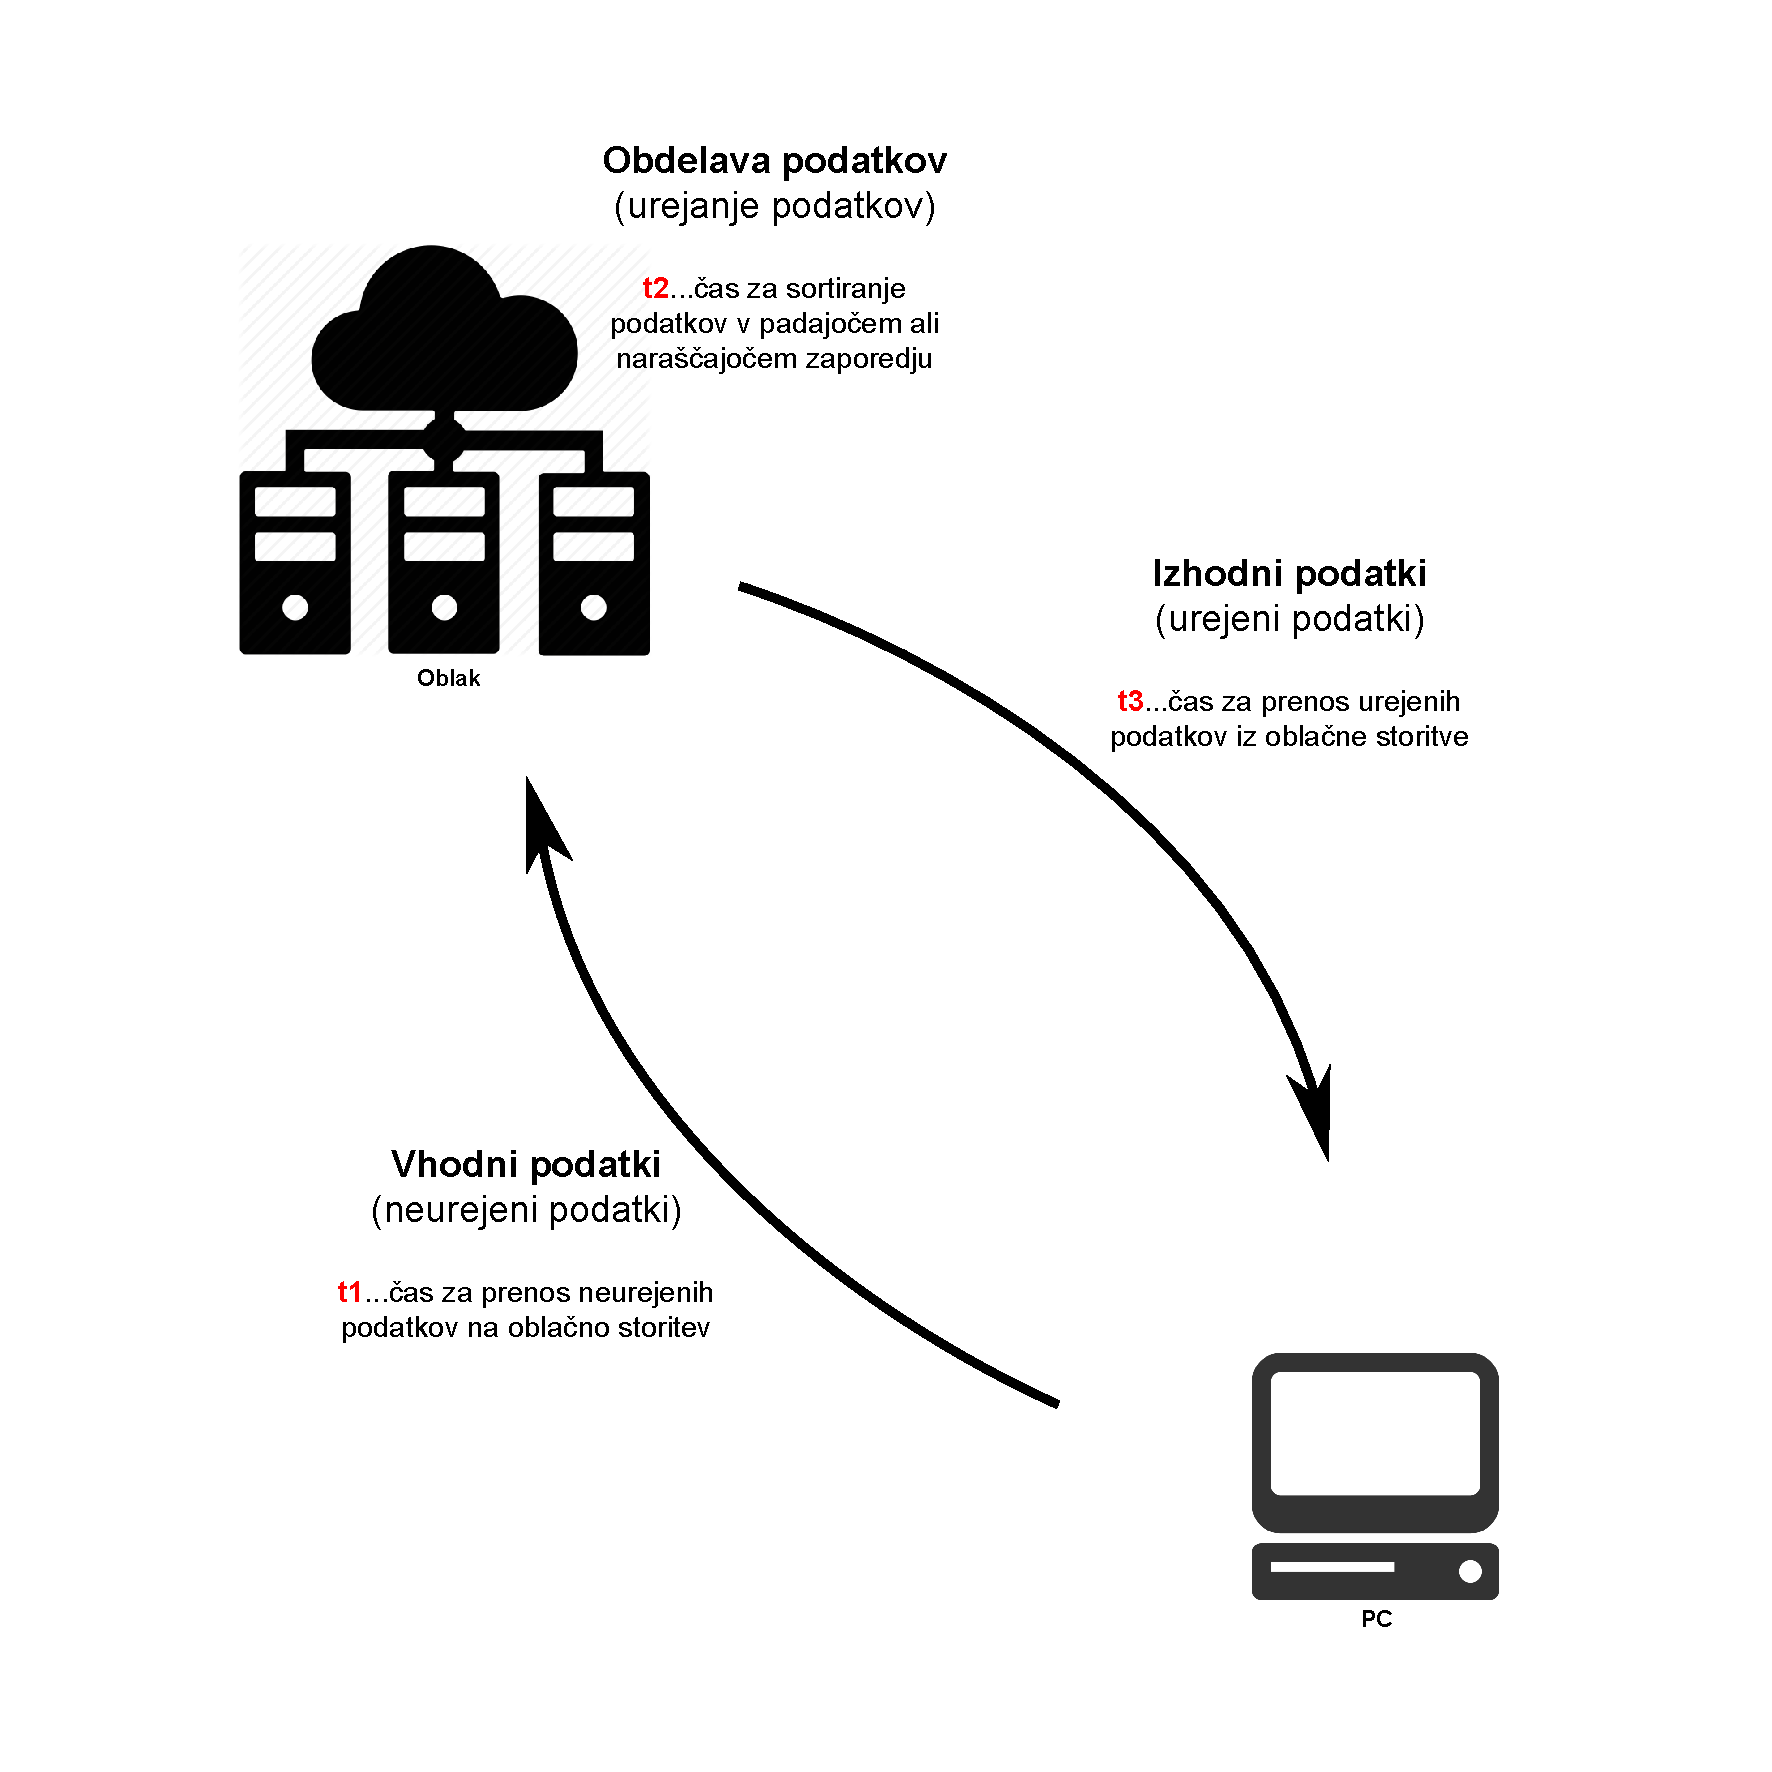
\includegraphics[width=0.74\textwidth]{8_zzrs_opis_problema.pdf}
  \caption{Shema delovanja sistema.}
  \label{8_opis_problema}
\end{figure}


\section{Izbira tehnologij in algoritmov}
V tem razdelku so opisane tehnologije in algoritmi, ki smo jih uporabili za na"so analizo.


\subsection{Tehnologija na strani stre"znika }
Na obla"cni stortivi smo implementirali stre"znik, ki je napisan v jeziku javascript (CITIRAJ JAVASCRIPT) z uporabo knji"znice Node.js. Stre"znik caka na HTTP zahtave. Ko stre"znik sprejme datoteko se za"cne izvajati program, ki "stevila v datoteki uredi po po vrsti. Ker je za ta program bistveno, da se izvede "cim hitreje smo za ta namen uporabili programski jezik C (CITIRAJ C), ki spada med najhitrej"se programske jezike. Po kon"canem sortiranju stre"znik urejeno datoteko po"slje nazaj odjemalcu. 

\subsection{Tehnologija za avtomatizacijo odjemalcev}
Zaradi avtomatskega testiranja smo napisali skripto v programskem jeziku python, ki omogo"ca avtomatsko po"siljanje datotek na stre"znik, ter po"caka na odgovor(datoteka z urejenimi "stevili). Seveda ob tem zabele"zimo "se "cas pred po"siljanjem zahteve in "cas po prejetju urejene datoteke, da dobimo celotni "cas potreben za to, da dobimo urejeno datoteko. Ker je odjemalcev lahko ve"cje "stevilo, smo ta problem re"sili z nitmi, kjer vsaka nit predstavlja enega odjemalca in po"silja zahteve na stre"znik, preko istega IP naslova.

\subsection{Generiranje vhodnih podatkov}
V programskem jeziku C smo napisali generator datotek, ki ustvari datoteko željene velikosti z naklju"cnimi "srevili. Za teste smo generirali datoteke velikosti: 10000, 20000, 30000, 40000 in 50000 "stevil tipa integer.

\begin{figure} [!h]
  \centering
    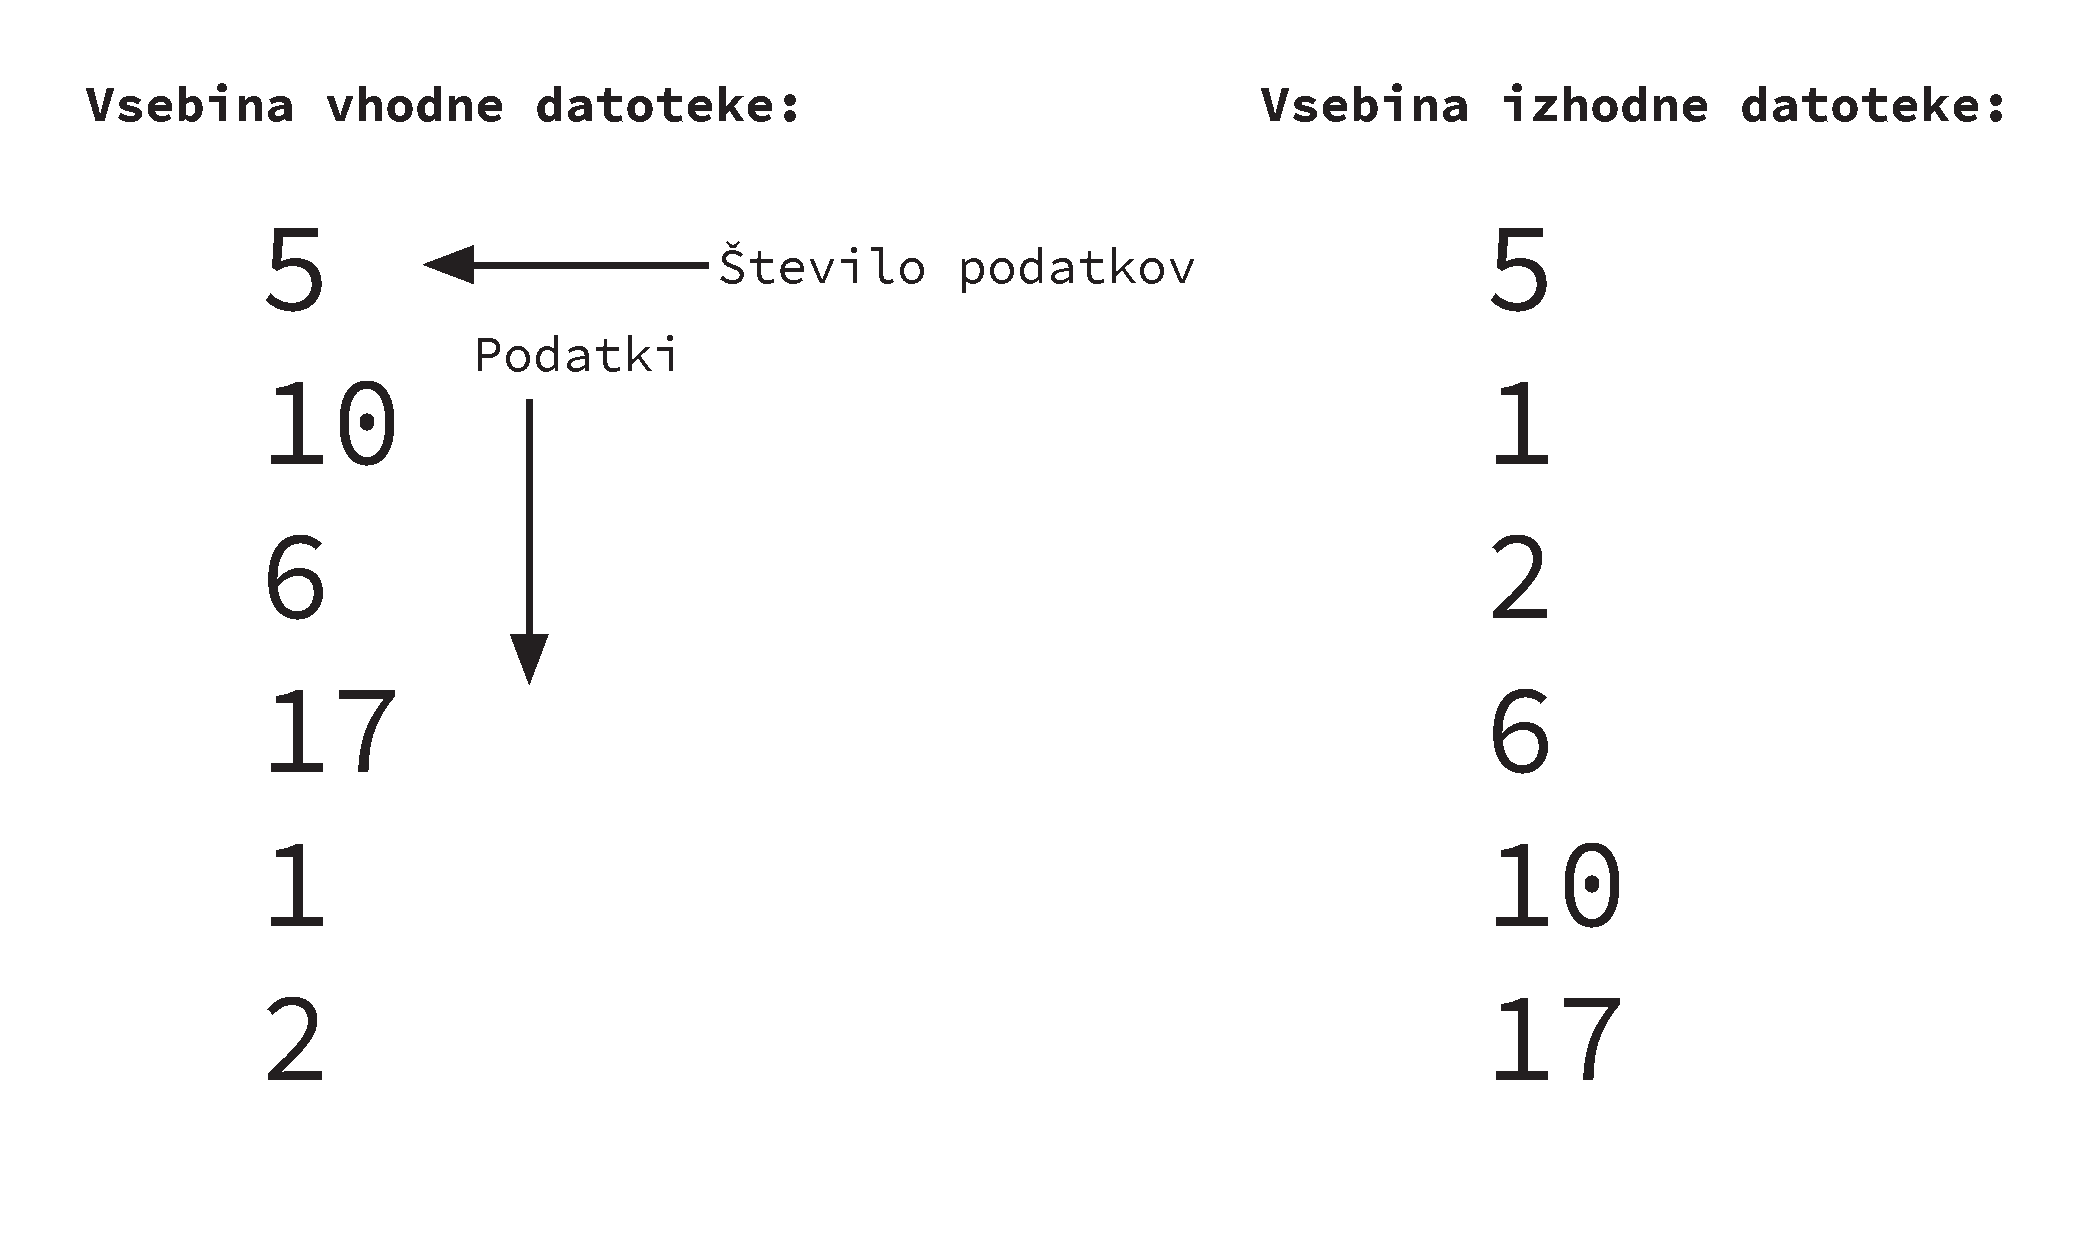
\includegraphics[width=0.75\textwidth]{ZZRS-sort_files.pdf} 
  \caption{Slika prikazuje primer datoteke s katero operirata stre"znik in odjemalec.}
  \label{8_files}  
\end{figure}

\subsection{Izbrani algoritmi za sortiranje}
Za namen testiranja smo implementirali dva algoritma. Najprej smo testirali z algoritmom za mehurčno urejanje(bubble sort), ki ima "casovno zahevnost $O(n^2)$.
Da bi testirali vpliv izbire algoritma smo implemenirali tudi algoritem quicksort z povpre"cno "casovno zahtevnostjo $O(n* log(n))$

\begin{figure}  [!h]
  \centering
    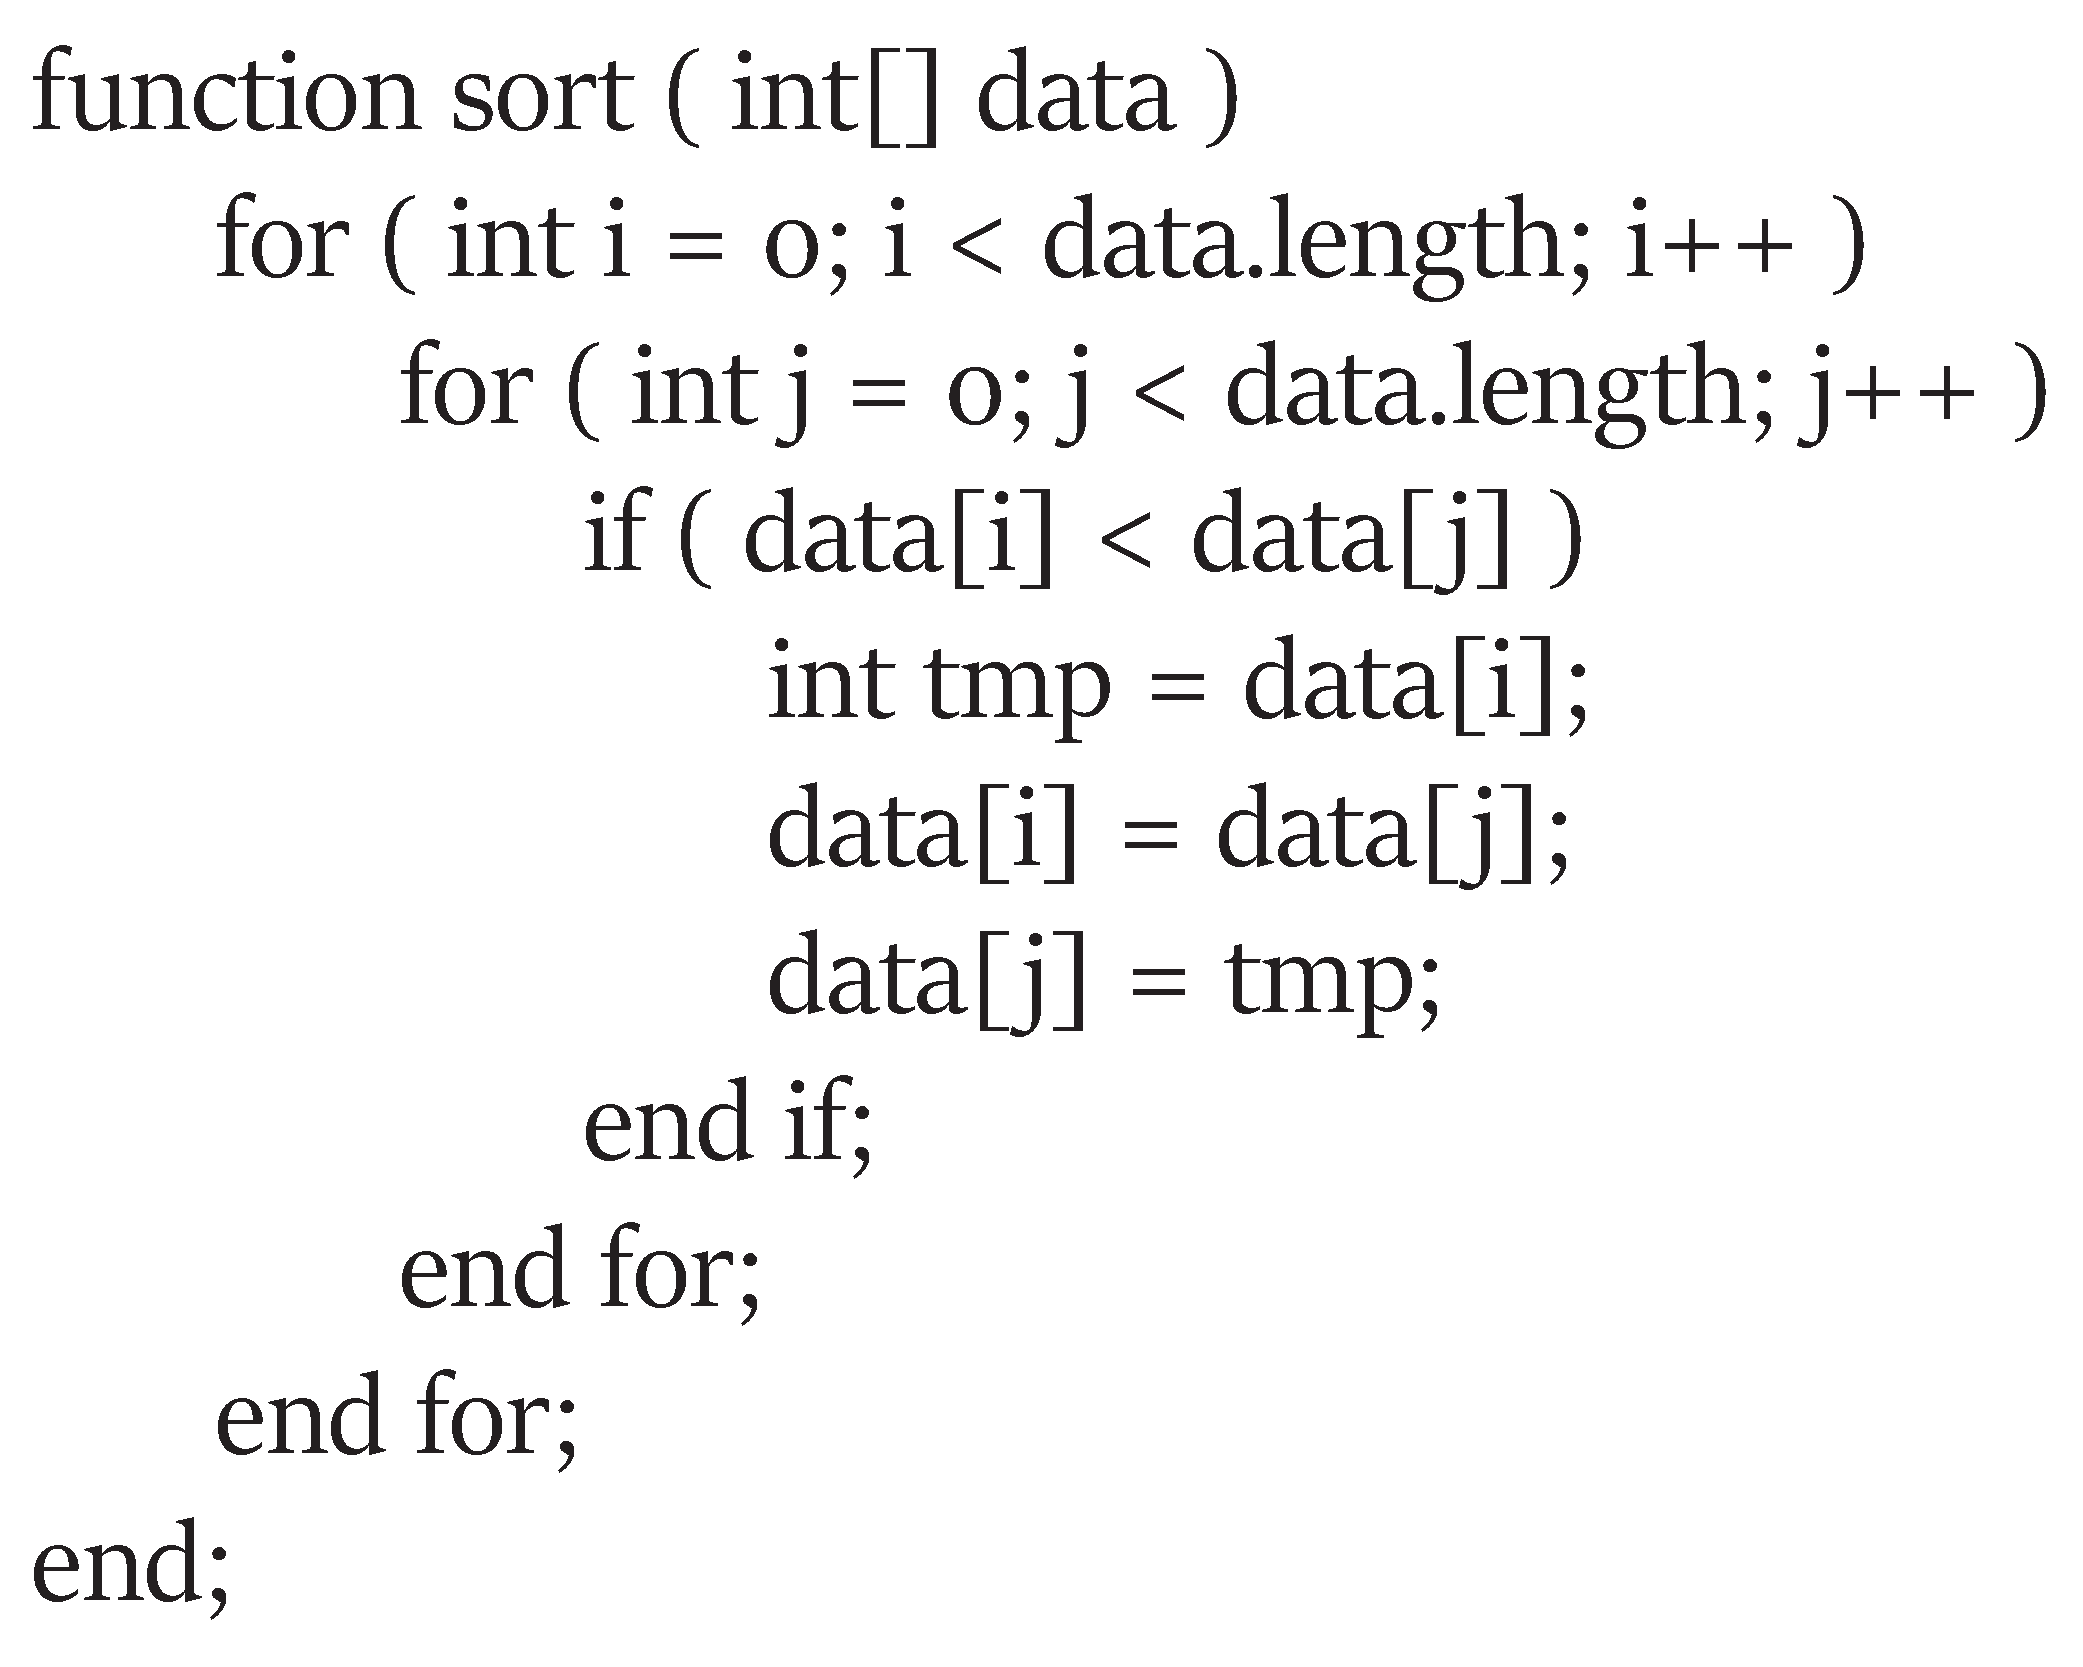
\includegraphics[width=0.65\textwidth]{ZZRS-sort_simple.pdf}
  \caption{Slika prikazuje algoritem sortiranja z $O(n^2)$ "casovno zahtevnostjo.}
  \label{8_sort}  
\end{figure}


\section{Izbira ponudnikov}
Najprej smo izbrali ponudnika obla"cnih storitev Cloud9, ki pa ni najbolj primeren za na"so nalogo, saj je v prvi vrsti razvojno okolje na spletu in ne toliko ponik stre"zniskih storitev. Pri ra"cunsko zahtevnej"sih testih smo naleteli na te"zave, saj je stre"znik po 120 sekundah povezavo zaprl. To je bil eden glavnih razlogov, da smo se odlo"cili zamenjati ponudnika, saj smo le tako lahko izvedli vse "zeljene teste. Izbrali smo ameri"sko podjetje DigitalOcean, ki je ponudnik istoimenske obla"cne infrastrukture. Na na"so sre"co sodelujejo v projektu Github Education Pack  in tako "studentom nudijo 50\$ kredita za uporabo njihovih storitev. Svoje stre"znike ima postavljene na osmih lokacijah po vsem svetu.
\begin{itemize}
\item New York (ZDA)
\item San Francisco (ZDA)
\item Amsterdam (Nizozemska)
\item Singapur (Singapur)
\item London (Zdru"zeno kraljestvo)
\item Fraknfurt (Nem"cija)
\item Bangalore (Indija)
\end{itemize}

V okviru "studentskih kreditv so nam na voljo tri razli"cne konfiguracije, ki se med seboj razlikujejo po koli"cini dodeljenih resursov.

\begin{figure}[!htbp]
  \centering
  \begin{tabular}{ | c | c | c | c | }
    \hline
    RAM & Stevilo procesorjev & Prostor na disku(SSD) & Cena na mesec\\ \hline
    512MB & 1     & 20GB &  5\$ \\ \hline
    1GB & 1 & 30GB & 10\$ \\ \hline
    2GB & 2 & 40GB & 20\$ \\ \hline
  \end{tabular}
  \caption{Konfiguracije stre"znikov, ki so na voljo za "studentske kredite.}
  \label{8_table1}
  \centering
\end{figure}




\section{Rezultati meritev}


\subsection{Stevilo odjemalcev - Eksperiment 1}
\begin{itemize}
	\item \textbf{Hipoteza: }  \\
		Na"sa hipoteza je, da se povpre"cen "cas "cakanja odjemalca pribli"zno linearno pove"cuje z ve"canjem stevila odjemalcev, ki hkrati po"siljajo datoteke na stre"znik.
			
	\item \textbf{Okoli"s"cine meritve: } \\
		Testiranje smo izvedli v "cetrtek 18.5.2017 med 21:00 in 21:30 na stre"zniku v Frankfurtu. Na stre"zniku je tekel operacijski sistem Linux Ubuntu 16.04. Na voljo smo imeli 512MB RAMa-, 1 procesor ter 20GB prostora na SSD trdem disku. Na stre"zniku je bil izbran algoritem za mehur"cno urejanje(bubble sort). Skripto za simulacijo odjemalcev smo pognali iz "studentskega naselja Ro"zna dolina(Ljubljana). Da dostop je bila uporabljna internetna povezana s hitrostjo 100Mbps. 
		Na stre"znik smo po"siljali datoteke, ki so vsebovale 20,000 "stevil tipa integer in merili "case pri 1, 10, 20, 30 in 40 odjemalcih.

 	\item \textbf{Rezultati meritve: }  \\
		
	\begin{figure}[!htb]
  	\centering
  	  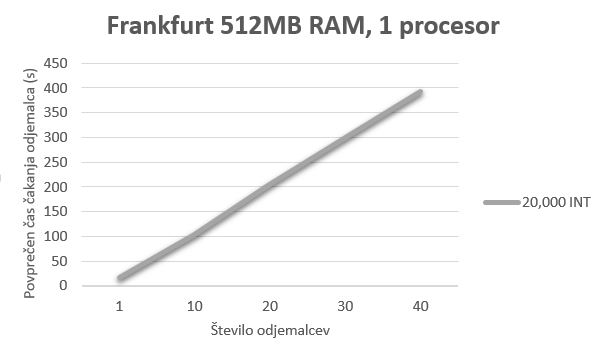
\includegraphics[width=1.0\textwidth]{test1_st_odjemalcev.jpg}
  	\caption{Graf povpre"cnega "casa cakanja odjemalcev v odvisnosti od "stevila odjemalcev.}
  	\label{8_graf_st_odjemalcev}
	\end{figure}

	\begin{figure}[!htbp]
  	\centering
  	\begin{tabular}{ | c | c | c | }
    	\hline
    	"Stevilo odjemalcev & Povpre"cni cas obdelave[s] & Standardna deviacija\\ \hline
    	1 & 16.059     & 0 \\ \hline
    	10 & 103.792 & 1.625\\ \hline
    	20 & 205.444 & 4.881\\ \hline
    	30 & 300.890 & 12.827\\ \hline
    	40 & 393.277 & 14.598\\ \hline
  	\end{tabular}
  	\caption{Tabela "casov obdelav datoteke z 20 tiso"c integer "stevili.}
  	\label{8_table1}
  	\centering
	\end{figure}

	\item \textbf{Komentar meritve: } \\ 
		Iz grafa lahko zelo razlo"cno vidimo, da se z ve"canjem "stevila odjemalcev linearno pove"cuje tudi povpre"cen "cas "cakanja posameznega odjemalca. To je rezultat, ki smo ga napovedali "ze v hipotezi, saj ima stre"znik omejeno "stevilo resursov in morajo zato ob ve"cjem stevilu zahtevkov odjemalci dlje "cakati. Prav tako lahko v tabeli opazimo, da se z ve"canjem stevila odjemalcev pove"cuje tudi standardna deviacija. To pomeni, da ob vi"sjih obremenitvah(ve"c odjemalcev) vedno te"zje predvidimo "cas obdelave datotek dolo"cenega klenta, saj prihaja do vedno ve"cjih odstopanj. 


\end{itemize}


\subsection{Velikost datotek - Eksperiment 2}
\begin{itemize}
	\item \textbf{Hipoteza: }  \\
		Z tem eksperimentom smo "zeleli preveriti odvisnost povpre"cnega "casa "cakanja klientov glede na velikost datotek. Da bi se izni"cili vpliv "stevila odjemalcev na ta poizkus smo teste ponovili na ve"c razli"cnih stevilih odjemalcev.
V tem primeru postavljamo hipotezo, da se z ve"canjem velikosti datoteke ve"ca tudi povpre"cni "cas "cakanja klientov. 
			
	\item \textbf{Okoli"s"cine meritve: } \\
		Testiranje smo izvedli v "cetrtek 18.5.2017 med 21:30 in 24:00 na stre"zniku v Frankfurtu. Na stre"zniku je tekel operacijski sistem Linux Ubuntu 16.04. Na voljo smo imeli 512MB RAMa-, 1 procesor ter 20GB prostora na SSD trdem disku. Na stre"zniku je bil izbran algoritem za mehur"cno urejanje(bubble sort). Skripto za simulacijo odjemalcev smo pognali iz "studentskega naselja Ro"zna dolina(Ljubljana). Da dostop je bila uporabljna internetna povezana s hitrostjo 100Mbps. 
	 Na stre"znik smo po"siljali datoteke, ki so vsebovale 10,000, 15,000, 20,000, 25,000, 30,000, 40,000 in 50,000 "stevil tipa integer. Meritve smo ponovili na 1, 10, 20, 30 in 40 odjemalcih.  

 	\item \textbf{Rezultati meritve: }  \\
		TODO: Zagotovi, da bo graf 1.7 tule..
		\begin{figure}[!h]
  		\centering
  		  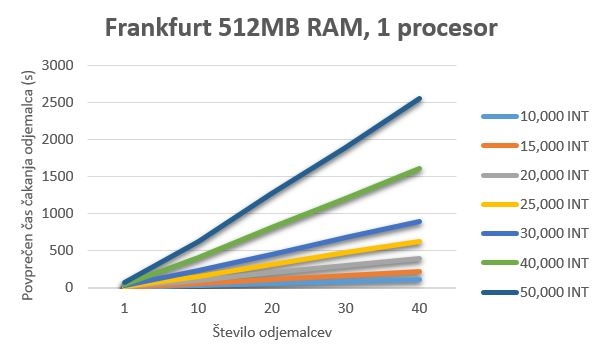
\includegraphics[width=1.0\textwidth]{test2_velikost_datotek.jpg}
  		\caption{Graf povpre"cnega "casa cakanja odjemalcev v odvisnosti od velikosti datotek.}		
  		\label{8_graf_st_odjemalcev}
		\end{figure}

	\item \textbf{Komentar meritve: } \\ 
		Iz grafa zelo razlo"cno vidimo, da se povpre"cen "cas "cakanja posameznega odjemalca z ve"canjem velikosti datotek zelo hitro pove"cuje. Pri 40 odjemalih in datoteki velikosti 10,000 stevil tipa integer je povpre"cni "cas cakanja pribli"zno 170 s. Pri datoteki veliosti 50,000 stevil pa ta "cats zna"sa "ze ve"c kot 2550 s. To je bilo pri"cakovano, saj je uporabljen algoritem za mehur"cno urejanje(bubble sort), ki ima "casovno zahtevnost  $O(n^2)$. Rezultati tega eksperimenta potrdijo, da se tudi na oblaku potreben "cas za obdelavo datotek z algoritmom bubble sort pove"cuje pribli"zno z kvadratom velikosti datotek. 
		


\end{itemize}

\subsection{Ozko grlo na stre"zniku - Eksperiment 3}
\begin{itemize}
	\item \textbf{Hipoteza: }  \\
		Z na"simi meritvami smo stre"znike obremenili do najvi"sjih dovoljenih meja. V praksi ob maksimani obremenitvi sistema vedno obstaja neko ozko grlo sistema, ki ne more delovati hitreje in z tem postavlja neko mejo hitrosti delovanja sistema. V na"sem primeru predpostavljamo, da je najbolj obremenjena komponenta procesor, saj je sortiranje operacija, ki zahteva relativno veliko ra"cunske mo"ci. 
			
	\item \textbf{Okoli"s"cine meritve: } \\
		Obrementive stre"znika smo merili med Eksperimentom 2 (LINK). 

 	\item \textbf{Rezultati meritve: }  \\
	TODO: Zagotovi, da bo graf tule
		\begin{figure}[!htb]
  		\centering
  		  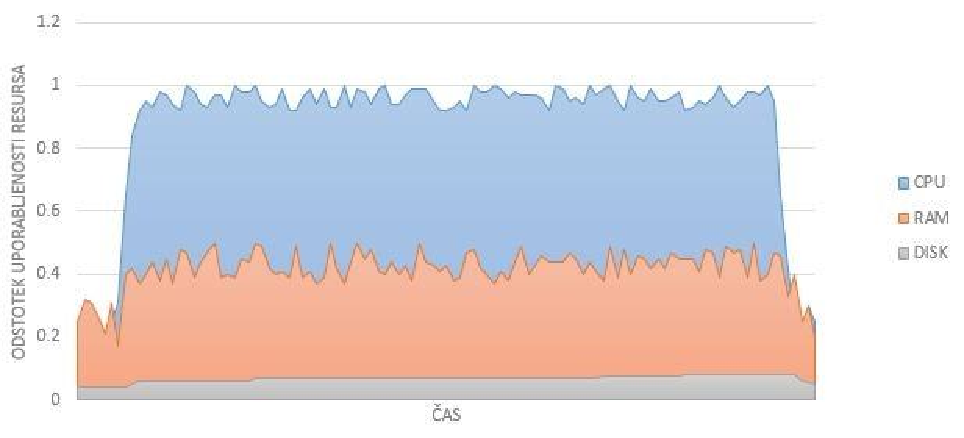
\includegraphics[width=1.0\textwidth]{test3_resursi.pdf}
  		\caption{Graf zasedenosti resursov med izvajanem testovs.}
  		\label{8_graf_zasedenost_resursov}
		\end{figure}


	\item \textbf{Komentar meritve: } \\ 
		Iz grafa (LINK) lahko razlo"cno razberemo, da je ozko frlo na"sega sistema procesor, saj je prakti"cno ves "cas izvajanja testov 100% obremenjen. Poraba RAM-a in kapacitete trdega diska niso nikoli ekstremo obremenjene, saj med izvajanem nikoli uporabljamo 50% RAM-a. Zasedenost diska pa je prakti"cno zanemarljiva, saj so datoteke relativno majhne glede na ponujeno velikost trgeda diska, datoteke pa se sproti bri"sejo in tako prepre"cimo te"zave z zasedenostjo trdega diska. 


\end{itemize}

\subsection{Lokalnost - Eksperiment 4}
\begin{itemize}
	\item \textbf{Hipoteza: }  \\
		Zaradi mo"znosti izbire lokacije stre"znika smo hoteli preveriti vpliv lokacije na povpre"cni "cas "cakanja odjemalcev. Poleg stre"znika v Frankfurtu smo vzpostavili tudi stre"znik v San Franciscu. Na"sa hipoteza je, da bomo hitrej"se odzive dobivali od stre"znika v Frankfurtu, saj nam je fizi"cno precej bli"zje, kot San Francisco.
			
	\item \textbf{Okoli"s"cine meritve: } \\
		Stre"znika imata dodeljeno enako kolic"cino resursov in name"sceno identi"cno programsko opremo. Ta je enaka kot v testu 2 (TODO: LINK) To je bilo potrebno zagotoviti, da izklju"cimo vpliv programske opreme na hitrost odzivov stre"znika. Testiranje smo izvedli v "ponedeljek 22.5.2017 med 10:00 in 14:00 po "casu UTC+01:00. Zaradi "casovnih pasov je bila ura v San Franciscu v "casu testiranja med 1:00 in 5:00 zjutraj. Teste smo ponovili z datotekami velikosti 20,000 in 50,000 celih stevil. 

 	\item \textbf{Rezultati meritve: }  \\
		TODO: zagotovi, da bosta oba grafa tule.
		\begin{figure}[!h]
  		\centering
  		  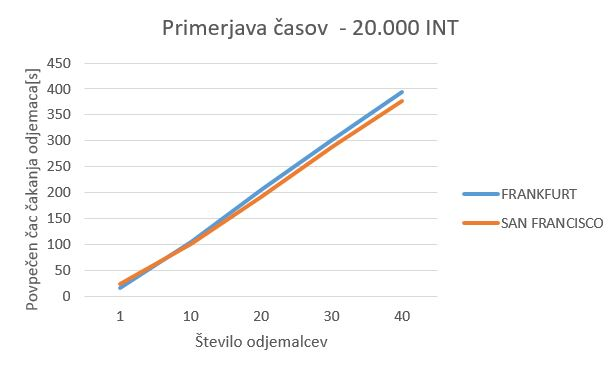
\includegraphics[width=1.0\textwidth]{test4_lokalnost_20.jpg}
  		\caption{Graf povpre"cnega "casa cakanja odjemalcev v odvisnosti od lokacije na primeru datoteke z 20,000 "stevili}
  		\label{8_graf_lokanlost_20}
		\end{figure}

		\begin{figure}[!h]
  		\centering
  		  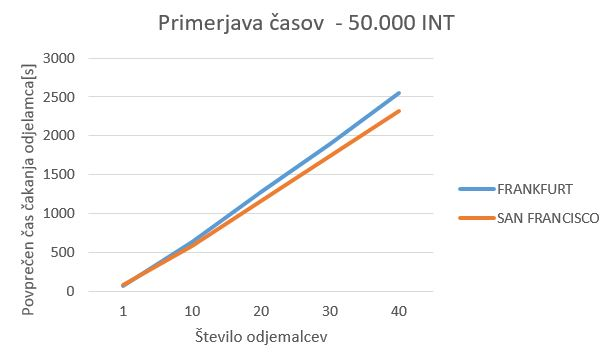
\includegraphics[width=1.0\textwidth]{test4_lokalnost_50.jpg}
  		\caption{Graf povpre"cnega "casa cakanja odjemalcev v odvisnosti od lokacije na primeru datoteke z 50,000 "stevili}
  		\label{8_graf_lokalnost_50}
		\end{figure}

	\item \textbf{Komentar meritve: } \\ 
		Rezultati meritev niso potrdili na"se hipoteze, saj je je stre"znik v San Franciscu kljub ve"cji oddaljenosti hitreje odzival in vra"cal urejene datoteke. 
		Razlike so vse bolj opazne bo ve"ci obremenitvi sistema (ve"cje datoteke in ve"c odjemalcev). Pri datoteki velikost 20,000 "stevil in enem odjemalcu lahko vidimo, da nam rezultate hitreje vrne stre"znik Frankfurtu. Rezultate si razlagamo na na"cin, da je bil stre"znik v Frankfurtu bolj obremenjen v "casu izvajanja testov. Pri majhnih primerih je kljub svoji obremenjenosti uspel rezultat vrniti pred stre"znikom v San Franciscu. Z ve"canjem ra"cunske zahtevnosti problema pa je vse bolj do izraza pri"sla manj"sa zasedenost infrastruktire v San Franciscu. Drug mo"zen razlog bi bili lahko zmoglivej"si procesorjiv stre"znikihv lociranih  v San Franciscu, vendar interne informacije o zgradbi stre"zni"skih centrov "zal niso javne.


\end{itemize}

\subsection{Razli"cne ra"cunske mo"ci - Eksperiment 5}
\begin{itemize}
	\item \textbf{Hipoteza: }  \\
		Na"sa hipoteze, ki jo bomo prevelili v tem poizkusu je, da se povpre"cni "cas "cakanja odjemalcev bistveno zmanj"sa, "ce je stre"znik bolj zmogljiv.
			
	\item \textbf{Okoli"s"cine meritve: } \\
		Testiranje smo izvedli v "torek 23.5.2017 med 00:30 in 02:30 na stre"zniku v Frankfurtu. Na stre"zniku je tekel operacijski sistem Linux Ubuntu 16.04. Na voljo smo imeli 2 GB RAM-a ter 2 procesorja. Na stre"zniku je bil izbran algoritem za mehur"cno urejanje(bubble sort). Skripto za simulacijo odjemalcev smo pognali iz "studentskega naselja Ro"zna dolina(Ljubljana). Da dostop je bila uporabljna internetna povezana s hitrostjo 100Mbps. 
		Na stre"znik smo po"siljali datoteke, ki so vsebovale 20,000 in 50,000 "stevil tipa integer in merili "case pri 1, 10, 20, 30 in 40 odjemalcih.

 	\item \textbf{Rezultati meritve: }  \\
		V spodnjig grafih so vizualizani "povpre"cni casi odziva treh razli"cnih streznikov. Streznik Frankfurt1 in San Francisco imata identi"cno konfiguracijo, kot je opisana v eksperimentu N (LINK). Stre"znik Frankfurt2 pa ima na voljo 2 procesorja ter 2GB RAM-a. 
		\begin{figure}[!h]
  		\centering
  		  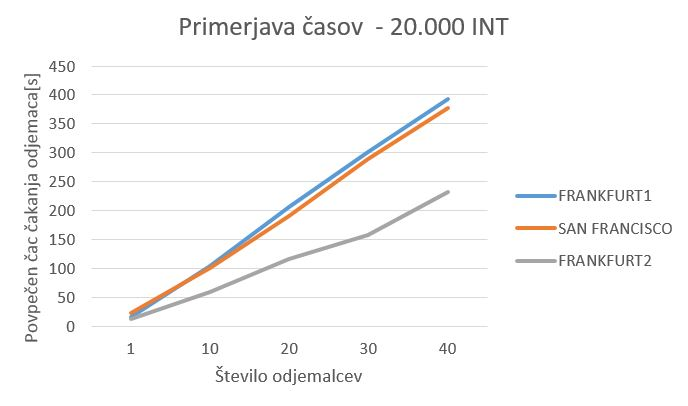
\includegraphics[width=1.0\textwidth]{test5_racunska_moc_20.jpg}
  		\caption{Graf povpre"cnega "casa cakanja odjemalcev treh razi"cnih stre"znikov na primeru datotek z 20,000 "stevili.}
  		\label{8_graf_racunska_moc_20}
		\end{figure}

	\begin{figure}[!h]
  		\centering
  		  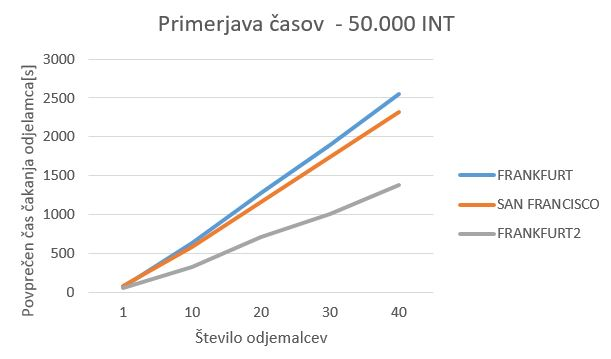
\includegraphics[width=1.0\textwidth]{test5_racunska_moc_50.jpg}
  		\caption{Graf povpre"cnega "casa cakanja odjemalcev treh razi"cnih stre"znikov na primeru datotek z 50,000 "stevili.}
  		\label{8_graf_racunska_moc_50}
		\end{figure}

	\item \textbf{Komentar meritve: } \\ 
		Meritve potrdijo na"so predpostavko, da vi"sja zmogljivst stre"znikov pripomore k bistveno ni"zjih povpre"cnih "casih potrebnih za odziv.



\end{itemize}




\iffalse

\subsection{Stevilo klientov - Eksperiment n}
\begin{itemize}
	\item \textbf{Hipoteza: }  \\
		To opi"semo kaj smo hoteli z meritvijo preveriti in kaj predpostalvjamo
			
	\item \textbf{Okoli"s"cine meritve: } \\
		Tu opi"semo kje, kdaj in kako smo meritev izvedli

 	\item \textbf{Rezultati meritve: }  \\
		Tu so rezultat meritve

	\item \textbf{Komentar meritve: } \\ 
		Tole je pa moj komentar meritve


\end{itemize}



\fi











